%%%%%%%%%%%%%%%%%%%%%%%%%%%%%%%%%%
% Felix Hoffmann, October 2014
% adapted from Jyotika Bahuguna October 2012
%%%%%%%%%%%%%%%%%%%%%%%%%%%%%%%%%%


%\documentclass{beamer}
\documentclass[xcolor=table,10pt]{beamer}
\usepackage{latexsym,amssymb,amsfonts,amsmath}
\usepackage{graphicx}
\usepackage{caption}
\usepackage{minted}
\usepackage{hyperref}

%for Introduction - Part 1 - ... Orientation
%\useoutertheme[subsection=false, shadow]{miniframes} 
\useinnertheme{default}
\beamertemplatenavigationsymbolsempty

\usefonttheme{serif}
\usepackage{palatino}
\usepackage{eulervm} %additional math 


% Other Palatino font packages, with math
% see also http://tex.stackexchange.com/questions/89610
% and math_fonts.pdf in Latex docs
% --------------------
% \usepackage{pxfonts}
% \usepackage{mathpazo} % add possibly `sc` and `osf` options
% --------------------

\setbeamercolor*{structure}{fg=black}

\usepackage{transparent} % transparent graphics

\usepackage{textcomp}
\usepackage{subcaption}
\graphicspath{{img/}{../}}

\usepackage[table]{xcolor}
\usepackage{tikz}
\usetikzlibrary{arrows,shapes}
\usepackage{color}

%\usemintedstyle{friendly}
%\usemintedstyle{autumn}
%\usemintedstyle{manni}
%\usemintedstyle{tango}

\newminted[mlinepython]{python}{fontsize=\small, linenos,
               		numbersep=11pt,
               		gobble=4,
               		frame=lines,
                        bgcolor=bg,
               		framesep=3mm}    



% http://tex.stackexchange.com/questions/84936/
\usepackage[loadonly]{enumitem} % Enumitem-Beamer Incompatibility! See
                                % http://tex.stackexchange.com/a/52299/4912
\newlist{arrowlist}{itemize}{1}
\setlist[arrowlist]{label=$\Rightarrow$}


\usepackage[english]{babel}
\usepackage[latin1]{inputenc}




\newenvironment{mydescription}[1]                                               
  {\begin{list}{}%
   {\renewcommand\makelabel[1]{\textbf{##1}\hfill}%
   \settowidth\labelwidth{\makelabel{#1}}%
   \setlength\leftmargin{\labelwidth}
   \addtolength\leftmargin{\labelsep}}}
  {\end{list}}

% cite source for content in the frame in bottom right corner
% usage: \source{here my source}
\usepackage[absolute,overlay]{textpos}
\setbeamercolor{framesource}{fg=gray}
\setbeamerfont{framesource}{size=\scriptsize}
\newcommand{\source}[1]{\begin{textblock*}{5cm}(7.7cm,8.9cm)
    \begin{beamercolorbox}[ht=0.5cm,right]{framesource}
        \usebeamerfont{framesource}\usebeamercolor[fg]{framesource} {#1}
    \end{beamercolorbox}
\end{textblock*}}

%%%%%%%%%%%%%%%%%%%%%%% stretching %%%%%%%%%%%%%%%%%%%%%%%%%%%%%%%

% from http://tex.stackexchange.com/questions/148365 
% and https://gist.github.com/navarroj/7789910

\let\svpar\par
\let\svitemize\itemize
\let\svenditemize\enditemize
\let\svitem\item
\def\newpar{\def\par{\svpar\vfill}}
\def\newitem{\def\item{\vfill\svitem}}
\let\svcenter\center
\let\svendcenter\endcenter
\let\svcolumn\column
\let\svendcolumn\endcolumn
\newlength\columnskip
\columnskip 0pt
\def\newcolumn{%
  \renewenvironment{column}[2]%
    {\svcolumn{##1}\setlength{\parskip}{\columnskip}##2}%
    {\svendcolumn\vspace{\columnskip}}}

\newcommand\stretchy{\only<2>{%
  \newpar\def\item{\svitem\newitem}%
  \renewenvironment{itemize}{\svitemize}{\svenditemize\newpar\par}%
  \renewenvironment{center}{\svcenter\newpar}{\svendcenter\newpar}%
  \newcolumn
}}

%%%%%%%%%%%%%%%%%%%%%%%%%%%%%%%%%%%%%%%%%%%%%%%%%%%%%%%%%%%%%%%%%%%%


\title {File operations, data parsing and batch files}
%\subtitle{}

\author[Felix Hoffmann]{Felix Hoffmann} 
\institute[BCF]{Bernstein Center Freiburg}
\date{\today}


\AtBeginSection[]
{
\begin {frame}<beamer>
\frametitle{}
\tableofcontents[currentsection]
\end{frame}
}


%%%%%%%%%%%%%%%%%%%%%%%%%%%%%%%%%%%%%%%%%%%%%%

\begin{document}

\definecolor{bg}{rgb}{0.95,0.95,0.95}
\definecolor{tg}{rgb}{0.35,0.35,0.35}










\section{Data parsing}

\begin{frame}{Need for parsing}
  % 
  \begin{columns}[T]
    %
    \begin{column}{.4\textwidth}
      Image that
      \vspace{0.5cm}
      \begin{arrowlist}
        \itemsep8pt
        \item[]<1-> Data files are generated by a third party (no control
          over the format)
        \item[]<2-> \& the data files need pre-processing
          \vspace{0.3cm}
        \item<3-> Regular expressions provide a powerful and concise way
          to perform pattern match/search/replace over the data
      \end{arrowlist}

    \end{column}
    %
    \begin{column}{.6\textwidth}
      \onslide<4->
      \begin{figure}
        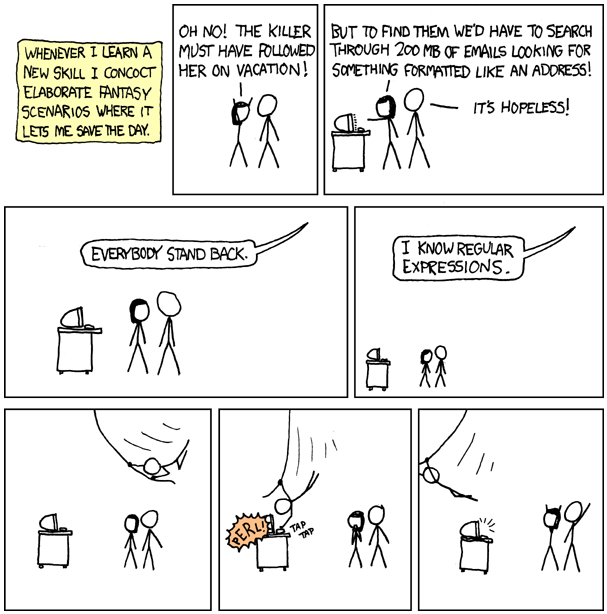
\includegraphics[width=6.4cm]{xkcd208.png}
        \caption*{\tiny  \textcopyright Randall Munroe \href{http://xkcd.com/208/}{xkcd.com} \href{http://creativecommons.org/licenses/by-nc/2.5/}{CC BY-NC 2.5}}
      \end{figure}
    \end{column}    

    %
  \end{columns}
  %
\end{frame}





% %%%%%%%%%%%%%%%%%%%%
\begin{frame}
\frametitle{Regex - A pratical introduction}
\begin{itemize}
\item Main challenge is to come up with a pattern using regex literals, that match the requirements of parsing.
\item Regex literals
	\begin{itemize}
		\item \^ - Matches beginning of line/pattern
		\item \$ - Matches end of line/pattern
		\item . - Matches any character except newline
		\item {[}..{]} - Matches any single character in brackets
		\item {[}\^..{]}- Matches any single character not in brackets
		\item re* - Matches 0 or more occurrences of the preceding expression
		\item re+ - Matches 1 or more occurrences of the preceding expression
		\item re? - Matches 0 or 1 occurrence
		\item re\{n\} - Match exactly n occurrences
		\item re\{n,\} - Match n or more occurrences
		\item re\{n,m\} - Match at least n and at most m
   	\end{itemize}
\end{itemize}
\end{frame}

%%%%%%%%%%%%%%%%%%%%
\begin{frame}[fragile]
\frametitle{Regex - re.search()}
\begin{itemize}
\item Suppose the pattern to match is "python"
\item regex module in python is "re"
\item re.search(pattern, string, flags=0) $\rightarrow$ matches the pattern in string\\

\begin{minted}{python}
import re
data = "I like python"
ans = re.search(r'python',data)
ans.group() # returns the entire match
Out[20]: 'python'
\end{minted}
\small
\item Suppose the pattern to match is "python" or "Python"\\

\begin{minted}{python}
data = "Python is a programming language. I like python"
ans = re.search(r'[pP]ython',data)
ans.group()
Out[38]: 'Python'
\end{minted}
\small
\item Though the regex is correct, re.search() returns as soon as it finds one instance.{[} re.findall() {]}
\item re.match((pattern, string, flags=0), same as search() but only at start of the string 
\end{itemize}
\end{frame}



%%%%%%%%%%%%%%%%%%%%
\begin{frame}[fragile]
\frametitle{Regex - re.findall()}
\begin{itemize}
\item re.findall(pattern, string, flags=0) $\rightarrow$ returns a list of all occurences of pattern\\

\begin{minted}{python}
data = "Python is a programming language. I like python"
ans = re.findall(r'[pP]ython',data)
print ans
['Python', 'python']
\end{minted}
\small
\item Suppose the aim is to extract all numbers from a data stream

\begin{minted}{python}
data = "There are 7 students and 2 tutors"\\
ans = re.findall(r'[0-9]+',data)\\
print ans
['7', '2']
\end{minted}
\small
(Note these are strings and need to be cast into integers for arthimetic operation)\\
\end{itemize}
\end{frame}



%%%%%%%%%%%%%%%%%%%%
\begin{frame}[fragile]
\frametitle{Regex - More examples}
\begin{itemize}
\item Suppose the aim is to extract strings not numbers

\begin{minted}{python}
data = "There are 7 students and 2 tutors"
ans = re.findall(r'[^ 0-9]+',data)
print ans
['There are ', ' students and ', ' tutors']
\end{minted}
\small
\item Multiple regular expressions can be used to perform the job. For eg,\\

\begin{minted}{python}
ans = re.findall(r'[a-zA-Z]+',data)
print ans
['There', 'are', 'students', 'and', 'tutors']
\end{minted}
\small
\item However slight difference. 
\end{itemize}
\end{frame}

%%%%%%%%%%%%%%%%%%%%
\begin{frame}[fragile]
\frametitle{Regex -  re.split()}
\begin{itemize}
\item Suppose the data stream has well-defined delimiter.\\

\begin{minted}{python}
data = "x = 20"
ans = re.split(r'=',data)
print ans
['x', '20']
\end{minted}
\vspace{1mm}
\begin{minted}{python} 
data = 'ftp://python.about.com'
ans = re.split(':/{1,3}', data)
print ans
['ftp', 'python.about.com']
\end{minted}
\small
\item Searching for regex literals as strings. Escape the meaning by a preceding backslash $\backslash$

\begin{minted}{python}
data = '25.657' # Split into whole and fractional parts
ans = re.split(r'\.',data)
print ans
['25', '657']
\end{minted}
\end{itemize}
\end{frame}

%%%%%%%%%%%%%%%%%%%%
\begin{frame}[fragile]
\frametitle{Regex -  re.sub()}
\begin{itemize}
\item Most powerful of them all.
\item re.sub(pattern, repl, string, max=0) looks for a pattern and replaces with repl
\item Aim is to delete python style comments in the line below:\\

\begin{minted}{python}
data = "2004-959-559 #This is Phone Number"
ans = re.sub(r'#.*','',data)
print ans
'2004-959-559 '
\end{minted}
\small
\item Now delete the hyphens from the above phone number.\\

\begin{minted}{python}
ans1 = re.sub(r'-','',ans)
print ans1
'2004959559 '
\end{minted}
\end{itemize}
\end{frame}

%%%%%%%%%%%%%%%%%%%%
\begin{frame}
\frametitle{Regex - Some shortcuts}
\begin{itemize}
\item $\backslash$w - Matches word character 
\item $\backslash$W - Matches non-word character
\item $\backslash$s - Matches whitespace (Equivalent to $\backslash$t$\backslash$n$\backslash$r," ")
\item $\backslash$S - Matches non-whitespace.
\item $\backslash$d - Matches digits (Equivalent to {[}0-9{]} )
\item $\backslash$D - Matches non digits
\item $\backslash$A - Matches beginning of the string
\item $\backslash$Z - Matches end of the string
\item $\backslash$B - Matches nonword boundaries
\item $\backslash$n,$\backslash$t - Matches newline, tab resp
\end{itemize}
\end{frame}




% %%%%%%%%%%%%% What are they? %%%%%%%%%%% 
% \section{Batch files}
% %%%%%%%%%%%%%%%%%%%%%%%%%%%%%%%%%%%%%%%%
% %%%%%%%%%%%%%%%%%%%%
% \begin{frame}[fragile]
% \frametitle{os module}
% \begin{itemize}
% \item Meta scripts that can automate your task
% \item os module in python provides a way of using os dependent functionality
% 	\begin{itemize}
% 	\item os.mkdir() - Creates a directory (like mkdir)
% 	\item os.chmod() - Change the permissions (like chmod)
% 	\item os.rename() - Rename the old file name with the new file name.\	
% 	\item os.listdir() - List the contents of the directory\
% 	\end{itemize}
% \item batch file batch\_file.py to run your script exercise.py for all data files in a directory.\\
% 
% \begin{minted}{python}
% from os import listdir
% files = listdir(".")
% for f in files: 
% 	os.system('python exercise.py f')
% \end{minted}
% \end{itemize}
% \end{frame}

% %%%%%%%%%%%%%%%%%%%%
% \begin{frame}
% \frametitle{Summary}
% \begin{itemize}
% \item Using these libraries, a lot of workflow can be automated.
% \item One doesnt require to learn something separate for pre-processing, processing and automation. Python does it all.
% \end{itemize}

% Suggestion for exercises:
% Test your regex on the file "regextest.gdf" first.\\ It is a reduced version of data files(only 100 data points).\\
% Hence visual inspection can be used easily to check if regex worked correctly.
% \end{frame} 




\end{document}

